\documentclass[11pt,a4paper]{article}
\usepackage[utf8]{inputenc}
\usepackage[T1]{fontenc}
\usepackage{amsmath}
\usepackage{amsfonts}
\usepackage{amssymb}
\usepackage{geometry}
\usepackage{hyperref}
\usepackage{enumitem}

\usepackage{graphicx}
\usepackage{subcaption}
\usepackage{setspace}

\onehalfspacing

\geometry{margin=2.5cm}

\title{Informe: resolución del entorno Taxi-v4 mediante Q-Learning}
\author{
    José Aviani \\
    \texttt{jose.aviani@gmail.com}
    \and
    Ricardo Silvera \\
    \texttt{rsilvera@thalu.com.ar}
    \and
    José Luis Diaz \\
    \texttt{diazjoseluis@gmail.com}
}
\date{\today}

\begin{document}

\maketitle

\section{Introducción y descripción del problema}

El problema del "Taxi" es un entorno clásico de Reinforcement Learning. Se desarrolla en una grilla de $5 \times 5$ donde un agente (el taxi) debe recoger a un pasajero en una de cuatro localizaciones específicas, denotadas por sus colores en inglés (R: Rojo, G: Verde, Y: Amarillo, B: Azul), y transportarlo hacia un destino determinado dentro de esas mismas opciones.

Para ilustrar la variabilidad del entorno, en la Figura \ref{fig:taxi_configs} se presentan tres configuraciones de estado inicial generadas aleatoriamente. Donde se pueden ver las locaciones especificas, que representan inicio y fin. Asimismo podemos ver la locación aleatoria del taxi.

\begin{figure}[h!]
    \centering
    \begin{subfigure}[b]{0.3\textwidth}
        \centering
        
\includegraphics[width=\textwidth]{taxi_conf1.png}
        \caption{Pasajero en G, destino en Y.}
        \label{fig:conf1}
    \end{subfigure}
    \hfill
    \begin{subfigure}[b]{0.3\textwidth}
        \centering
        
\includegraphics[width=\textwidth]{taxi_conf2.png}
        \caption{Pasajero en R, destino en G.}
        \label{fig:conf2}
    \end{subfigure}
    \hfill
    \begin{subfigure}[b]{0.3\textwidth}
        \centering
        
\includegraphics[width=\textwidth]{taxi_conf3.png}
        \caption{Pasajero en Y, destino en B.}
        \label{fig:conf3}
    \end{subfigure}
    \caption{Ejemplos de distintos estados iniciales en la grilla de $5 \times 5$.}
    \label{fig:taxi_configs}
\end{figure}


\subsection{Desglose del Espacio de Estados (500 estados)}

Un aspecto fundamental del entorno Taxi-v4 es su espacio de estados discreto, el cual se compone de 500 combinaciones únicas. Estos estados se derivan de la multiplicación de tres variables independientes:

\begin{enumerate}
    \item \textbf{Posición del Taxi ($5 \times 5 = 25$):} la grilla cuenta con 25 celdas posibles donde el vehiculo puede estar ubicado.
    \item \textbf{Ubicación del Pasajero (5):} existen 4 localizaciones fijas (R, G, Y, B). A estas se suma un quinto estado que representa al pasajero cuando ya se encuentra dentro del taxi.
    \item \textbf{Destino (4):} Hay 4 localizaciones de destino posibles (R, G, Y, B).
\end{enumerate}

Matematicamente, el espacio total se define como:
\[ \text{Total de Estados} = 25 \text{ (posiciones)} \times 5 \text{ (pasajero)} \times 4 \text{ (destino)} = 500 \]

La codificacion interna del estado en \texttt{gymnasium} sigue la formula:
\[ S = ((f \times 5 + c) \times 5 + p) \times 4 + d \]
Donde $f$ es la fila, $c$ la columna, $p$ el estado del pasajero y $d$ el destino.

\section{Abordaje de la Solución: Q-Learning}

Para este desafío, se decidió implementar \textbf{Q-Learning}. La elección de este enfoque responde al interés de experimentar con un modelo \textbf{off-policy} sobre un problema de complejidad intermedia. 
Si bien Taxi-v4 opera sobre la base de un \textit{gridworld} clásico de dimensiones reducidas, la inclusión de variables lógicas (como el estado del pasajero y el destino) eleva la cardinalidad del espacio a 500 estados. Esto representa un incremento sustancial en la complejidad algorítmica respecto a entornos introductorios y puramente espaciales como \textit{FrozenLake} o \textit{CliffWalking}, exigiendo un mayor rigor en la gestión de la tabla Q y en la estrategia de exploración del agente.

La ventaja teórica de este algoritmo \textit{off-policy} es que permite aprender una política óptima $\pi^*$ independientemente de las acciones exploratorias que el agente esté tomando en el entorno. La actualización de la función de valor de acción $Q(s, a)$ se rige por la ecuación:

\[ Q(s, a) \leftarrow Q(s, a) + \alpha \left[ r + \gamma \max_{a'} Q(s', a') - Q(s, a) \right] \]

Para complementar la actualización de estos valores, la selección de acciones se rige por una política $\epsilon$-\textit{greedy} con decaimiento exponencial (\textit{epsilon decay}). En las etapas tempranas del entrenamiento, la matriz $Q(s,a)$ carece de información útil al inicializarse con valores nulos. Emplear una tasa de exploración estática y conservadora (por ejemplo, $\epsilon = 0.1$) fuerza al agente a "explotar" sistemáticamente una tabla vacía. Como el operador $\max$ resuelve empates entre ceros de forma arbitraria, el modelo navega con ineficiencia y sin una verdadera cobertura del entorno. Esto retrasa drásticamente el descubrimiento de la recompensa dispersa de $+20$.

\section{Implementación y Código Fuente}

La implementación se ha realizado íntegramente en \textbf{Python}, utilizando la biblioteca \texttt{gymnasium}. El script está diseñado para ser modular y eficiente, omitiendo el renderizado gráfico durante las fases de entrenamiento masivo para optimizar los tiempos de ejecución y el consumo de recursos.

El código fuente completo se encuentra disponible en el siguiente repositorio:

\begin{center}
    \url{https://github.com/jose/PostgradoIAUBA/CEIA-ApR-I/}
\end{center}

Para garantizar la correcta reproducibilidad de los resultados, el repositorio incluye un archivo \texttt{README.md} en su directorio principal. Este documento detalla los requisitos previos del sistema, el proceso de instalación de las dependencias necesarias, y las instrucciones precisas para la ejecución del algoritmo de entrenamiento en un entorno local.

\section{Inconvenientes encontrados y soluciones}

Durante el desarrollo se identificaron los siguientes desafíos:

\begin{itemize}
    \item \textbf{Propagación incorrecta en estados Terminales:} en las primeras pruebas, la ecuación clásica sumaba el valor futuro $\max_{a'} Q(s', a')$ incluso tras finalizar el episodio. Como en un MDP episódico el valor de un estado terminal es cero, esta sobreestimación se corrigió con una máscara lógica. Al multiplicar el término futuro por $(1 - \text{terminated})$. No se observó una gran diferencia entre incluir este valor, por esto no se incluyo el grafico, se puede ver en el repositorio de código.
        
    \item \textbf{Ruido en la convergencia:} la posición inicial aleatoria del taxi produce picos de varianza que dificultan evaluar el progreso del aprendizaje. Se aplicó una media móvil sobre la curva de recompensas para lograr una visualización clara y estable de la convergencia asintótica.
    
    \item \textbf{Mínimos locales en la exploración:} un decaimiento muy rápido del factor $\epsilon$ llevó al agente a adoptar políticas subóptimas, como inmovilizarse para evitar penalizaciones continuas de $-10$. Se ajustó el \textit{epsilon-decay} a un ritmo más gradual para forzar una exploración exhaustiva del entorno antes de explotar la tabla Q.
\end{itemize}

\section{Análisis de resultados y convergencia}

\begin{figure}[h!]
    \centering
    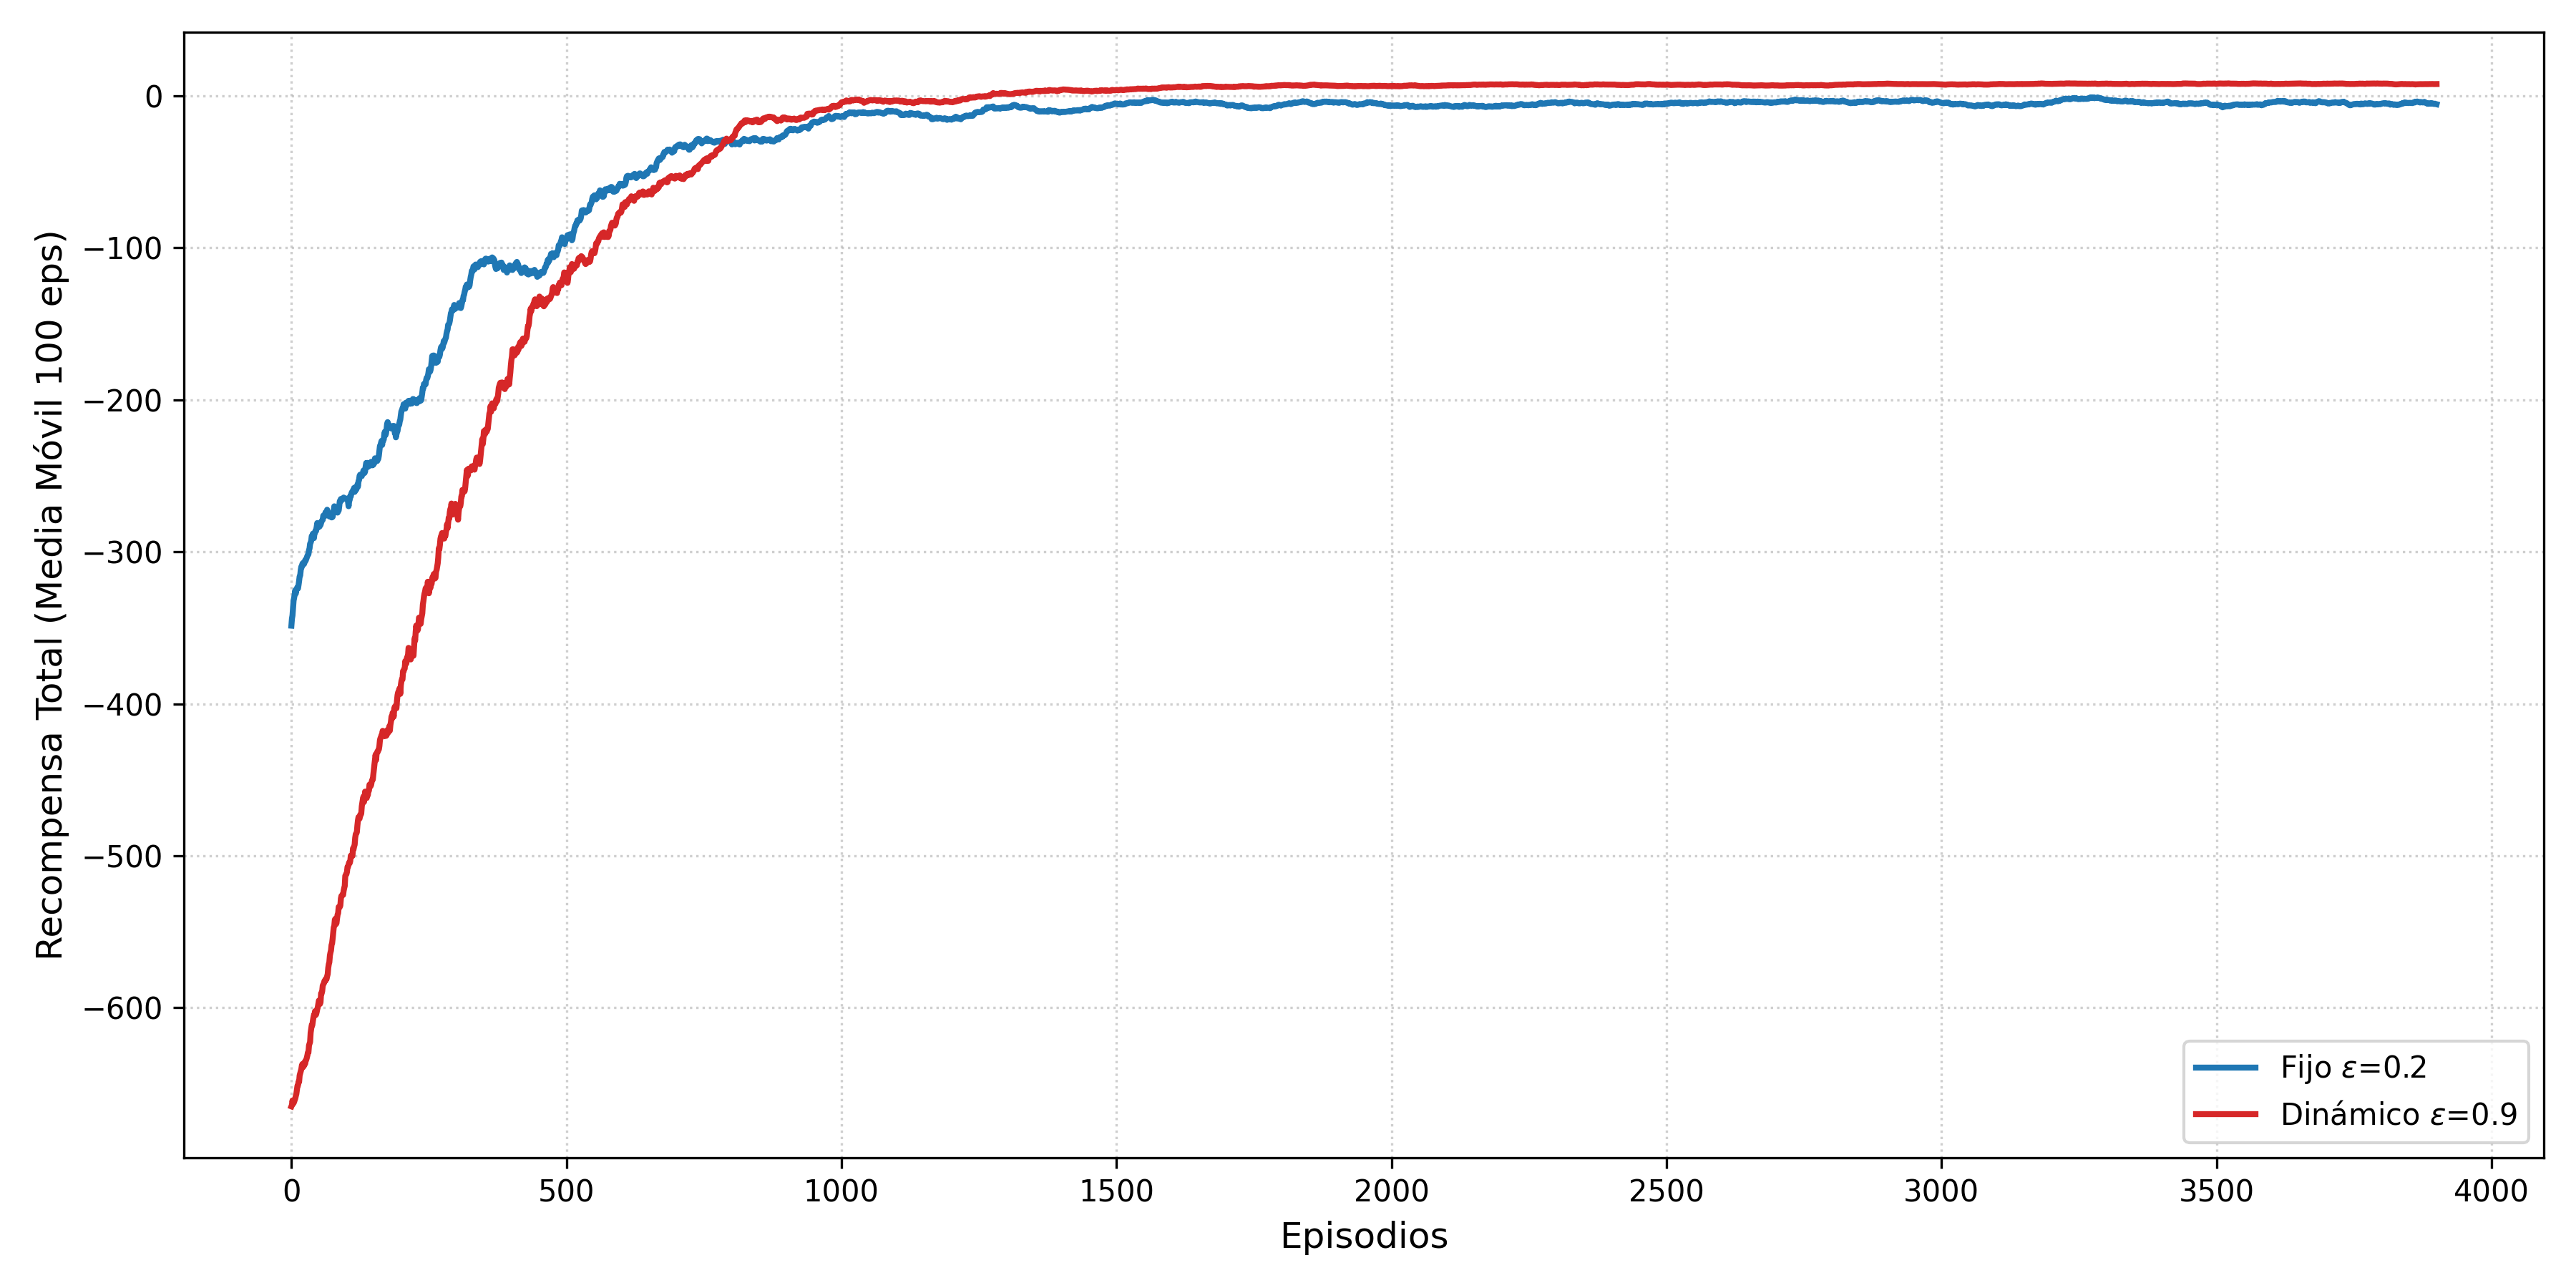
\includegraphics[width=0.85\textwidth]{comparativa_epsilon.png}
    \caption{Curva de convergencia del agente en Taxi-v4.}
    \label{fig:comp}
\end{figure}


El proceso de aprendizaje y el impacto de la estrategia de exploración fueron evaluados mediante el seguimiento de la recompensa acumulada por episodio. En la Figura \ref{fig:comp} se presenta el gráfico comparativo obtenido tras 4.000 episodios de entrenamiento, contrastando un agente con decaimiento dinámico de $\epsilon$ (iniciando en $0.9$) frente a uno con tasa estática ($\epsilon = 0.2$).

Como se evidencia en la comparativa, la utilización de un $\epsilon = 0.9$ inicial con decaimiento progresivo resulta en un desempeño cualitativa y cuantitativamente superior. Este enfoque dinámico fuerza al agente a barrer el espacio de estados en su totalidad durante los primeros episodios, lo que le permite superar rápidamente las penalizaciones extremas. Al converger, el modelo alcanza y estabiliza una recompensa promedio óptima de $+8.0$ a $+8.5$, demostrando haber consolidado la política ideal para resolver el entorno en el mínimo número de pasos.

Por el contrario, el agente sujeto a una tasa estática moderada ($\epsilon = 0.2$) arroja un rendimiento significativamente inferior a lo largo de toda la corrida. Al dedicar el 80\% de sus acciones iniciales a "explotar" una tabla Q inicializada en ceros, sus selecciones \textit{greedy} resultan arbitrarias y carentes de un mapeo previo del entorno. Esta deficiencia exploratoria inicial atrapa al modelo en un régimen de recompensas subóptimo, donde nunca logra igualar el puntaje asintótico del enfoque dinámico.


\end{document}
